%%
%%  chapter07.tex - Obstacle Detection and Planning for Autonomous Vehicles based on Computer Vision Techniques
%%
%%  Copyright 2014 Néstor Morales <nestor@isaatc.ull.es>
%%
%%  This work is licensed under a Creative Commons Attribution 4.0 International License.
%%

\graphicspath{{./images/chapter07/bmps/}{./images/chapter07/vects/}{./images/chapter07/}}

\chapter{Local Planning}\label{ch:chapter07}

% Intro:
% Path planning allows an autonomous vehicle to determine the behavior of a vehicle by itself.
% 
% Ya tenemos un conocimiento exhaustivo del entorno del vehículo y una ruta global que conecta su posición con la del punto de destino
% Con esta ruta global por sí sola no hacemos nada, ya que no modela la impredictibilidad del entorno a largo plazo, ya que este entorno es cambiante debido a la presencia de obstáculos móviles.
% Además necesitamos un mecanismo que nos permita seguir la trayectoria.
% 
% Muchos de estos métodos de generación trayectorias se basan en un esquema de optimización discreta:
% 
% Un cjto finito de paths es calculado:
% + reduce el espacio de soluciones y
% + permite una implementación de tiempo real 
% 
% 
% Habitualmente esto se hace mediante forward integration de las ecuaciones diferenciales que describen la dinamica del vehiculo
% Del cjto de trayectorias se escoge aquella que minimiza un det. coste
% Para la generacion de trayectorias un modelo parametrico es empleado, habitualmente func. polinomiales de un orden arbitratio. 
% Nosotros usamos splines calculados sobre el espacio de frenet
% 
% 
% La ruta global forma un base frame de un sistema de coordenadas curvilineo que es el espacio de generacion de las paths
% 
% La info. direccional de la ruta global es incorporada a la de maniobras del vehiculo ajustando el offset lateral al base frame
% 
% El trabajo está inspirado en el sistema desarrollado por los coreanos y stanley
% 
% - empleamos un base frame
% - generamos rutas candidatas basadas en la posición actual respecto al base frame y una serie de endpoints en posiciones fijadas a diferentes offsets respecto al base frame
% - Cada ruta es evaluada cuantitativamente mediante una funcion de coste
%   + Al igual que en Stanley, nosotros usamos la distancia al centro de la ruta como funcion de coste
%     ++ A diferencia suya, el centro de la ruta no es calculado mediante un metodo basado en filtros de Kalman, sino el metodo basado de multiclass SVM descrito en el capitulo anterior
%   + Al igual que los coreanos, nuestra funcion de coste se basa en la suavidad de la ruta y el coste de chocar con los obstaculos calculado como una funcion de distancia a los mismos
%     ++ Sin embargo, en nuestro caso este coste no se basa en el blurring de los datos binarios de un mapa de obstaculos
%       +++ Nosotros usamos un mapa de costes basados en una funcion exponencial relativa a la distancia y al footprint del vehículo
%   + Tambien usamos las funciones de coste...
% 
% Estas funciones de coste seran descritas con mayor detalle en la seccion XXX
% 
% En este trabajo nos hemos focalizado en la consecucion de resultados experimentales que logren el correcto funcionamiento de verdino a nivel practico, mas que en mejorar el algoritmo en si mismo, aunque aportamos algunas soluciones que mejoran los resultados iniciales al ser adaptado a las caracteristicas especiales de nuestro vehiculo.
% 
% El algoritmo resultante ha sido aplicado sobre verdino. Al final de este capitulo se muestran algunos resultados experimentales. Ademas, hay disponible una serie de videos que muestran el vehiculo en funcionamiento.
%   
% ===========================================================================
% Poner la parte de generacion del mapa de costes
%   Describir brevemente, esto mejor lo dejo para el ultimo capitulo
%   También hablar del rolling window(ultimo capitulo)
% Hablar de la parte de frenet
%   Decir que hay codigo disponible de esta parte concreta???
% 
%   \begin{figure}
% \begin{tabular}{cc}
% \subfloat{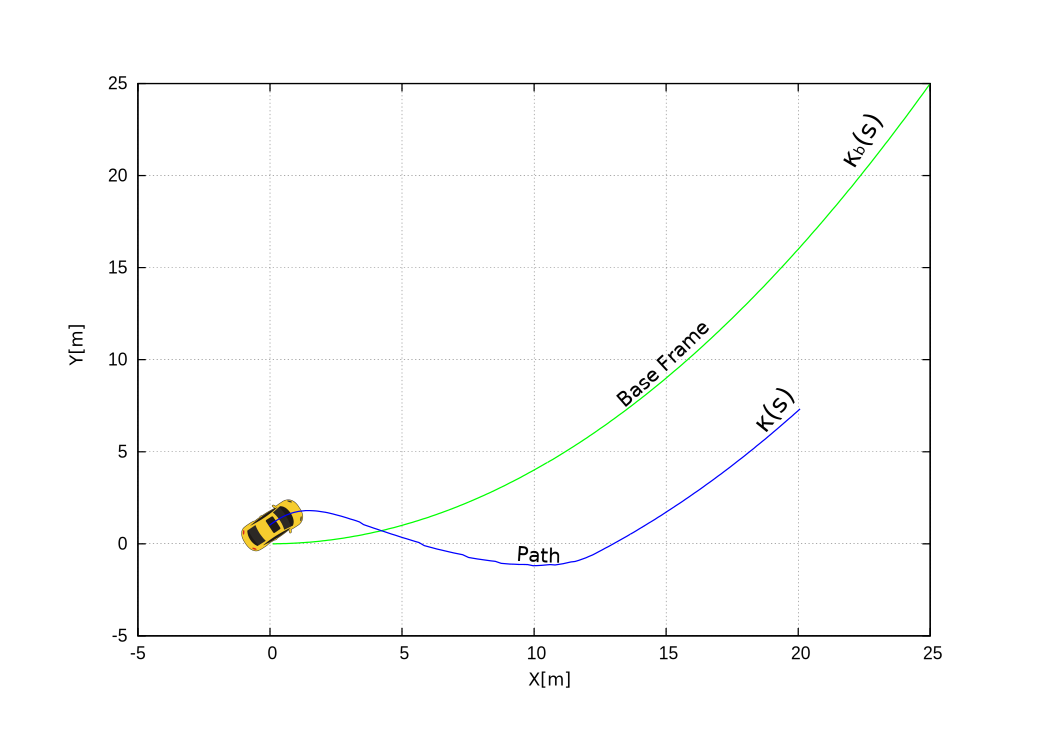
\includegraphics[width=0.5\textwidth,trim=50 40 80 60,clip]{justOneCartesian45}} &
% \subfloat{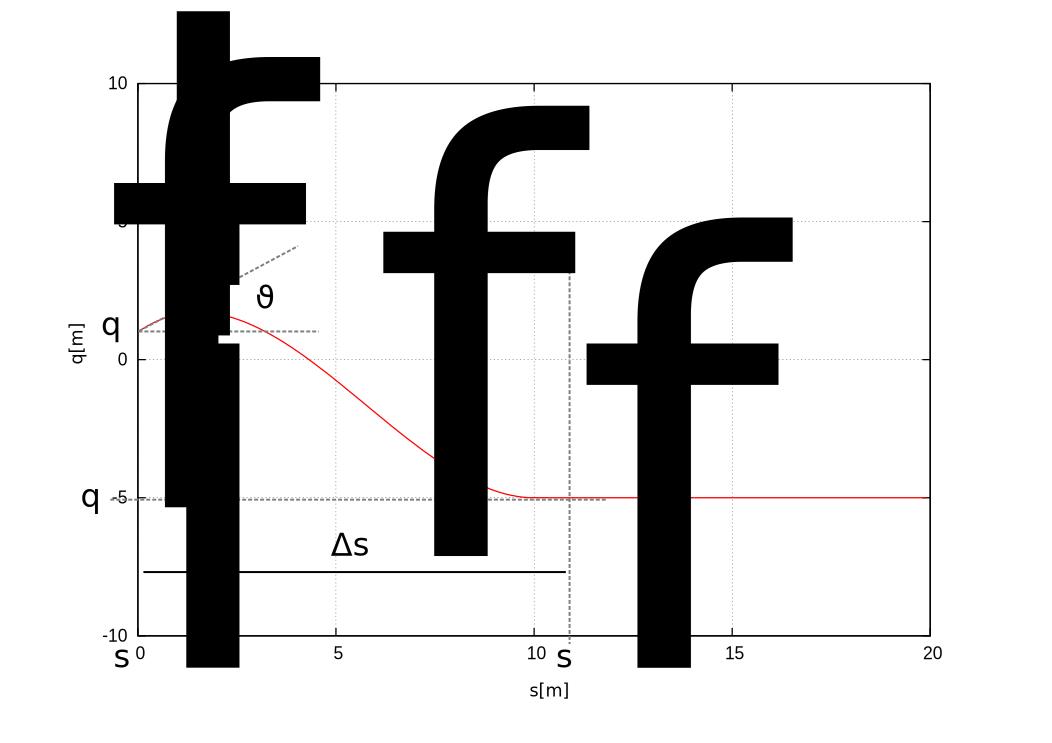
\includegraphics[width=0.5\textwidth,trim=50 40 80 60,clip]{justOneFrenet45}}
% \end{tabular}
% \caption{Conversion of a trajectory between the Cartesian and Frenét spaces. \todo{Incluir la información disponible en el paper original para estas figuras (9 y 10)}}\label{fig:cp07_cartesian_frenet_conversion}
% \end{figure}
% 
% \begin{figure}
% \begin{tabular}{cc}
% \subfloat{\includegraphics[width=0.5\textwidth,trim=50 40 80 60,clip]{cartesian0}} &
% \subfloat{\includegraphics[width=0.5\textwidth,trim=50 40 80 60,clip]{frenet0}}
% \end{tabular}
% \caption{Example in which the vehicle is oriented parallel to the path.}\label{fig:cp07_frenet0}
% \end{figure}
% 
% \begin{figure}
% \begin{tabular}{cc}
% \subfloat{\includegraphics[width=0.5\textwidth,trim=50 40 80 60,clip]{cartesian45}} &
% \subfloat{\includegraphics[width=0.5\textwidth,trim=50 40 80 60,clip]{frenet45}}
% \end{tabular}
% \caption{Example in which the vehicle is rotated with respect to the path.}\label{fig:cp07_frenet45}
% \end{figure}
  
% COSTES
% 
%   Asociar los originales con el paper de Corea
%   Asociar la distancia lateral con Stanley
%   Describir los nuevos costes
% 
% Consistency cost
% \begin{figure}
% \subfloat{\includegraphics[width=0.5\textwidth]{example3a}}\label{fig:cp07_consistency_frame1} ~~~
% \subfloat{\includegraphics[width=0.5\textwidth]{example3b}}\label{sdsgd}
% 
% \centering
% \subfloat{\includegraphics[width=0.5\textwidth,trim=50 40 80 60,clip]{consistency}}\label{fig:cp07_consistency_costs}
% \caption{Example of the costs obtained using the consistency cost.}\label{fig:cp07_examplesC}
% \end{figure}

%  Hablar de como calculamos la ruta final
%   Describir el modelo de la bicicleta

% RESULTADOS
% ===========================================================================  
%   Enlazar videos


% \subsection{Path following performance}\label{ch:XXX}
% 
% Se ha capturado la posición del vehículo en cada momento y se ha comparado con la posición más cercana dentro de la ruta global.
% No se ha permitido al planificador global replanificar en ningun momento.
% \begin{figure}[th]
%   \centering
%   \includegraphics[trim=50 50 90 60, clip]{differences}
%   \caption{Comparison between the localization of the vehicle and the nearest point in the global path.}\label{fig:cp07_localization_diff}
% \end{figure}
% 
% \subsection{Costs}\label{ch:XXX}
% 
% 
% \begin{figure}
% \begin{tabular}{cc}
% \subfloat{\includegraphics[width=0.5\textwidth]{example1}} &
% \subfloat{\includegraphics[width=0.5\textwidth,trim=50 40 80 60,clip]{costs1}}\label{fig:cp07_example1}\\
% \subfloat{\includegraphics[width=0.5\textwidth]{example2}} &
% \subfloat{\includegraphics[width=0.5\textwidth,trim=50 40 80 60,clip]{costs2}}\label{fig:cp07_example2}\\
% \subfloat{\includegraphics[width=0.5\textwidth]{example4}} &
% \subfloat{\includegraphics[width=0.5\textwidth,trim=50 40 80 60,clip]{costs4}}\label{fig:cp07_example3}\\
% \subfloat{\includegraphics[width=0.5\textwidth]{example5}} &
% \subfloat{\includegraphics[width=0.5\textwidth,trim=50 40 80 60,clip]{costs5}}\label{fig:cp07_example4}
% \end{tabular}
% % \caption{Some examples of the computed paths and their costs.}\label{fig:cp07_examplesA}
% \end{figure}
% 
% \begin{figure}
% \begin{tabular}{cc}
% \subfloat{\includegraphics[width=0.5\textwidth]{example12}} &
% \subfloat{\includegraphics[width=0.5\textwidth,trim=50 40 80 60,clip]{costs12}}\label{fig:cp07_example5}\\
% \subfloat{\includegraphics[width=0.5\textwidth]{example14}} &
% \subfloat{\includegraphics[width=0.5\textwidth,trim=50 40 80 60,clip]{costs14}}\label{fig:cp07_example6}\\
% \subfloat{\includegraphics[width=0.5\textwidth]{example15}} &
% \subfloat{\includegraphics[width=0.5\textwidth,trim=50 40 80 60,clip]{costs15}}\label{fig:cp07_example7}
% \end{tabular}
% \caption{Some examples of the computed paths and their costs.}\label{fig:cp07_examplesB}
% \end{figure}
% 
% \begin{figure}
% \begin{tabular}{cc}
% \subfloat{\includegraphics[width=0.5\textwidth]{example16}} &
% \subfloat{\includegraphics[width=0.5\textwidth,trim=50 40 80 60,clip]{costs16}}\label{fig:cp07_example8}\\
% \subfloat{\includegraphics[width=0.5\textwidth]{example17}} &
% \subfloat{\includegraphics[width=0.5\textwidth,trim=50 40 80 60,clip]{costs17}}\label{fig:cp07_example9}
% \end{tabular}
% \caption{Some examples of the computed paths and their costs.}\label{fig:cp07_examplesC}
% \end{figure}
% 
% \subsection{Obstacle avoidance}\label{ch:XXX}
% 
% \begin{figure}
% \begin{tabular}{cc}
% \subfloat{\includegraphics[width=0.5\textwidth]{example9}} &
% \subfloat{\includegraphics[width=0.5\textwidth]{seq9}}\label{fig:cp07_seq1}\\
% \subfloat{\includegraphics[width=0.5\textwidth]{example10}} &
% \subfloat{\includegraphics[width=0.5\textwidth]{seq10}}\label{fig:cp07_seq2}\\
% \subfloat{\includegraphics[width=0.5\textwidth]{example11}} &
% \subfloat{\includegraphics[width=0.5\textwidth]{seq11}}\label{fig:cp07_seq3}
% \end{tabular}
% \caption{Example of a sequence in which an obstacle is avoided.}\label{fig:cp07_sequence}
% \end{figure}

% Resumen
%   Hablar de las ventajas/desventajas
%   Indicar que en la fase siguiente se describe la integracion con los obstaculos detectados empleados por los metodos de los capitulos previos